\documentclass{article}

\usepackage{graphicx}

\begin{document}

	% 그림 삽입하기
	% option의 종류
	% width : 그림의 폭을 지정
	% height : 그림의 높이를 지정
	% angle : 그림을 반시계방향으로 회전
	% scale : 그림의 배율을 지정
	\begin{figure}
  		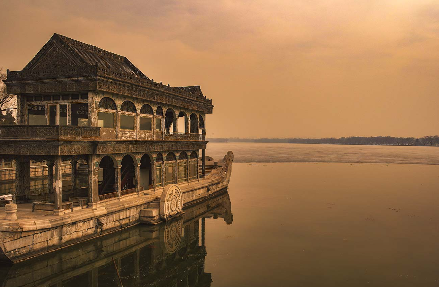
\includegraphics[width=\linewidth]{boat.png}
  		\caption{A boat(1).}
  		\label{fig:boat1}
	\end{figure}

Figure \ref{fig:boat1} shows a boat.

	% 그림 위치 지정하기
	% LaTeX의 경우 적절한 위치로 그림을 이동하므로, 
	% 특정한 위치를 원한다면 지정해야 함!
	% h(here), t(top), b(bottom), p(page), !(override)
	\begin{figure}[h!]
  		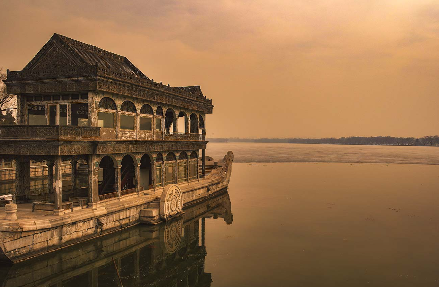
\includegraphics[width=\linewidth]{boat.png}
  		\caption{A boat(2).}
  		\label{fig:boat2}
	\end{figure}

\end{document}